\documentclass[polish]{article}

\title{Wykrywanie wdechu i wydechu na podstawie dźwięku z mikrofonu}
\author{Dominik Lau, Mateusz Kowalczyk, Michał Tarnacki}

\usepackage{blindtext}
\usepackage{amsmath}
\usepackage[utf8]{inputenc}
\usepackage[polish]{babel}
\usepackage[T1]{fontenc}
\usepackage{listings}
\usepackage{color}
\usepackage{amssymb}
\usepackage{esvect}
\usepackage{graphicx}
\usepackage{caption}
\usepackage{hyperref}
\usepackage{float}


\usepackage{etoolbox}
\patchcmd{\thebibliography}{\section*{\refname}}{}{}{}

\graphicspath{ {./obrazy/} }

\definecolor{dkgreen}{rgb}{0,0.6,0}
\definecolor{gray}{rgb}{0.5,0.5,0.5}
\definecolor{mauve}{rgb}{0.58,0,0.82}

\lstset{frame=tb,
  language=Python,
  aboveskip=3mm,
  belowskip=3mm,
  showstringspaces=false,
  columns=flexible,
  basicstyle={\small\ttfamily},
  numbers=none,
  numberstyle=\tiny\color{gray},
  keywordstyle=\color{blue},
  commentstyle=\color{dkgreen},
  stringstyle=\color{mauve},
  breaklines=true,
  breakatwhitespace=true,
  tabsize=3
}

\newcommand*{\captionsource}[2]{%
  \caption[{#1}]{%
    #1%
    \\\hspace{\linewidth}%
    \textbf{Źródło:} #2%
  }%
}



\begin{document}

\maketitle

\section{Wstęp}
Celem projektu było określanie chwil na nagraniu, w których osoba bierze wdech i wydech. 
Dokonano oceny jakościowej za pomocą detekcji oddechu na żywo jak i ilościowej (przy wykorzystaniu
dalej wymienionej metryk).

\section{Teoria}
\subsection{DFT}
W celu przejścia z dziedziny natężenia od czasu do dziedziny częstotliwości stosujemy dyskretną transformatę
Fouriera.  DFT przekształca ciąg skończonych próbek sygnału $a_0, a_1, a_2, ..., a_{N-1}$ w ciąg 
$A_1, ..., A_{N-1} \in \mathbb{C}$
\begin{gather*}
	A_k = \Sigma_{n=0}^{N-1} a_ne^{\frac{-kni\pi}{N}}, 0 \le k \le N-1
\end{gather*}
W naszych zastosowaniach będziemy brali pod uwagę tylko część rzeczywistą tego wielomianu
\begin{gather*}
	R_k = Re(A_k), 0 \le k \le N-1
\end{gather*}
Naszą funkcję natężenia w czasie dla pewnego okresu $t \in [t_0, t_0 + B]$, gdzie $B$ - rozmiar bloku (przyjmujemy $B=1024\approx \frac{1}{44} s$) przedstawiamy zatem jako 
\begin{gather*}
	I(t) = \Sigma_{f} I_{f}(t)sin(2 \pi f t)
\end{gather*}
stąd dla danego przedziału w czasie jesteśmy w stanie stworzyć wektor natężeń
\begin{gather*}
	\boldsymbol{I} = [I_{f_1}, I_{f_2}, ..., I_{f_n}]
\end{gather*}
W dalszych rozważaniach wykorzystujemy także średnią częstotliwość, którą liczymy ze wzoru
\begin{gather*}
	\bar{f} = \frac{\Sigma_ffI_f}{I}
\end{gather*}
Wykorzystujemy implementację transformaty z biblioteki $numpy$.
\subsection{Przeliczanie wyników DFT na częstotliwości}
TODO
\subsection{Bramka szumów}
Głowna metoda odszumiana, z której korzystamy to $Spectral$ $Gating$ (rodzaj bramki szumów).  Pierw wyznaczany jest spektrogram sygnału za pomocą $DFT$ i 
tworzony jest próg szumu dla każdej jego częstotliwości.
Częstotliwości progowe służą to stworzenia maski, której potem używamy do usunięcia niechcianych dźwięków.
Następnie ze spektrogramu tworzymy z powrotem natężenie $I(t)$. W projekcie wykorzystujemy gotową implementację bramki szumów z biblioteki $noisereduce$\footnote{\url{https://pypi.org/project/noisereduce/}}. Przykładowe wartości osiąganych SNR w porównaniu z innymi 
algorytmami usuwania szumu\footnote{źródła [3]}:
\begin{center}
\begin{tabular}{c  | c }
algorytm & SNR \\
\hline
$LMS$ & 2 \\
$Kalman$ & 6 \\
$Spectral$ $Gating$ & 14
\end{tabular}
\end{center}

\subsection{Filtr Savitzky-Golay}
Filtru Savitzky-Golay używamy do wygładzenia spektrogramu po przeprowadzeniu DFT.  Polega on na dopasowywaniu zbioru sąsiadujących punktów do wielomianu niskiego stopnia za pomocą metody najmniejszych kwadratów.
Te fragmenty wielomianów są potem łączone w wygładzoną funkcję. Korzystamy z gotowej implementacji
z biblioteki $scipy$.
\begin{figure}[H]
	\centering
	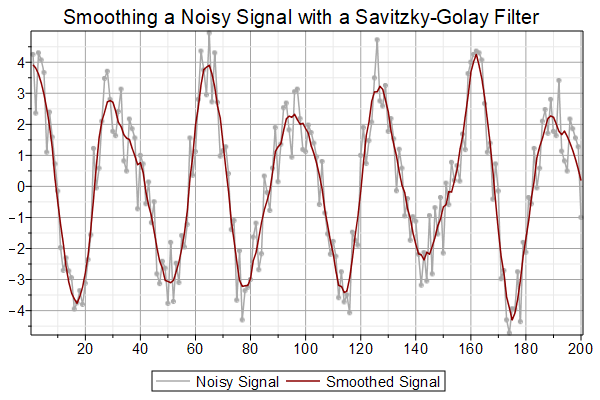
\includegraphics[width=10cm]{savitzky_golay_filter}
\end{figure}

\subsection{Ocena modeli}
Metryki oceny ilościowej modelu
\begin{gather*}
	accuracy = \frac{\# correct}{\# all} \\
	precision_{wdech} = \frac{\# correct_{wdech}}{\# correct_{wdech} + \# incorrect_{wdech}} \\
	recall_{wdech} = \frac{\# correct_{wdech}}{\# correct_{wdech} + \# incorrect_{wydech}} \\
	F_{wdech} = \frac{2 \cdot precision_{wdech} \cdot recall_{wdech}}{precision_{wdech} + recall_{wdech}}
\end{gather*}
analogiczne metryki $precision, recall, F$ definiujemy też dla wydechu
\subsection{Standaryzacja}
Dane wejściowe do modelu zawsze standaryzujemy, czyli
\begin{gather*}
	\tilde X = \frac{X - EX}{\sigma_X}
\end{gather*}
stosujemy gotową implementację z $scikit-learn$.
\subsection{SVM}
Pierwszym modelem, jakim dokonujemy klasyfikacji, jest SVM. Metoda ta polega na szukaniu optymalnych wag $\boldsymbol{w}, b$.
Następnie będziemy klasyfikować według funkcji maszyny uczącej 
\begin{gather*}
	f(x) = sgn(\boldsymbol{w}^T \boldsymbol{x} + b)
\end{gather*}
jeśli $f$ zwraca 1 to traktujemy to jako jedną z binarnych decyzji (w naszym przypadku np. wdech) a jeśli zwraca -1 to drugą (czyli np. wydech).
$\textbf{x}$ jest wektorem cech.  Znalezienie optymalnych wag będzie polegało na minimalizacji
funkcji kosztu
\begin{gather*}
	J(\boldsymbol{w}) = \frac{1}{2}||\boldsymbol{w}||^2 + \frac{C}{N}\Sigma_x max\{0, 1 - y(\boldsymbol{w}^Tx + b)\}
\end{gather*}
gdzie C jest parametrem uregulowania. Funkcję będziemy minimalizować metodą stochastycznego spadku po gradiencie.
W projekcie użyliśmy własnej implementacji SVM-a.
\section{Nagrywanie danych oddechowych}
Żeby zapewnić dobre oznaczenie danych, etykietujemy je jeszcze w trakcie nagrywania dźwięku. 
Osoba nagrywana naciska przycisk, żeby zasygnalizować, że przestała brać wdech i zaczyna wydychać 
powietrze lub na odwrót. Momenty przejścia z wdechu na wydech i w drugą stronę zapisywane są w pliku
.csv, a dźwięk w pliku .wav. Częstotliwość próbkowania ustalamy na $44,1$ kHz.
\begin{figure}[H]
	\centering
	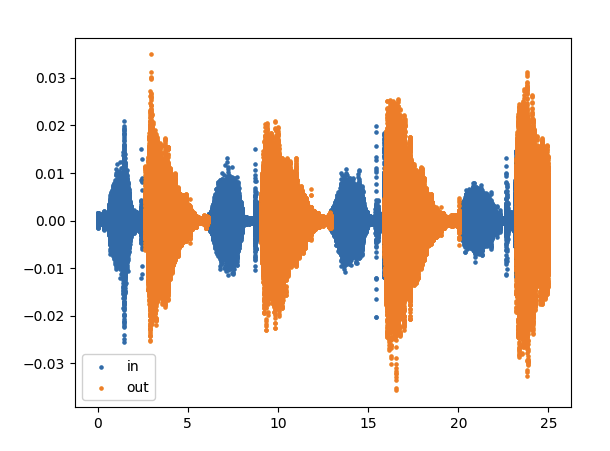
\includegraphics[width=10cm]{nagrywanie}
	\caption{Przykładowe nagrane dane, in-wdech, out-wydech. Jak widać dane oznaczone na żywo są bardzo dokładne, być może nie bylibyśmy w stanie osiągnąć takiej
dokładności oznaczając ręcznie (lub byłoby to bardzo żmudne).}
\end{figure}
\section{Oddychanie na żywo}
Testowanie modeli do predykcji na żywo odbywało się za pomocą programu wizualizującego aktualnie
stwierdzany stan. 
\begin{figure}[H]
	\centering
	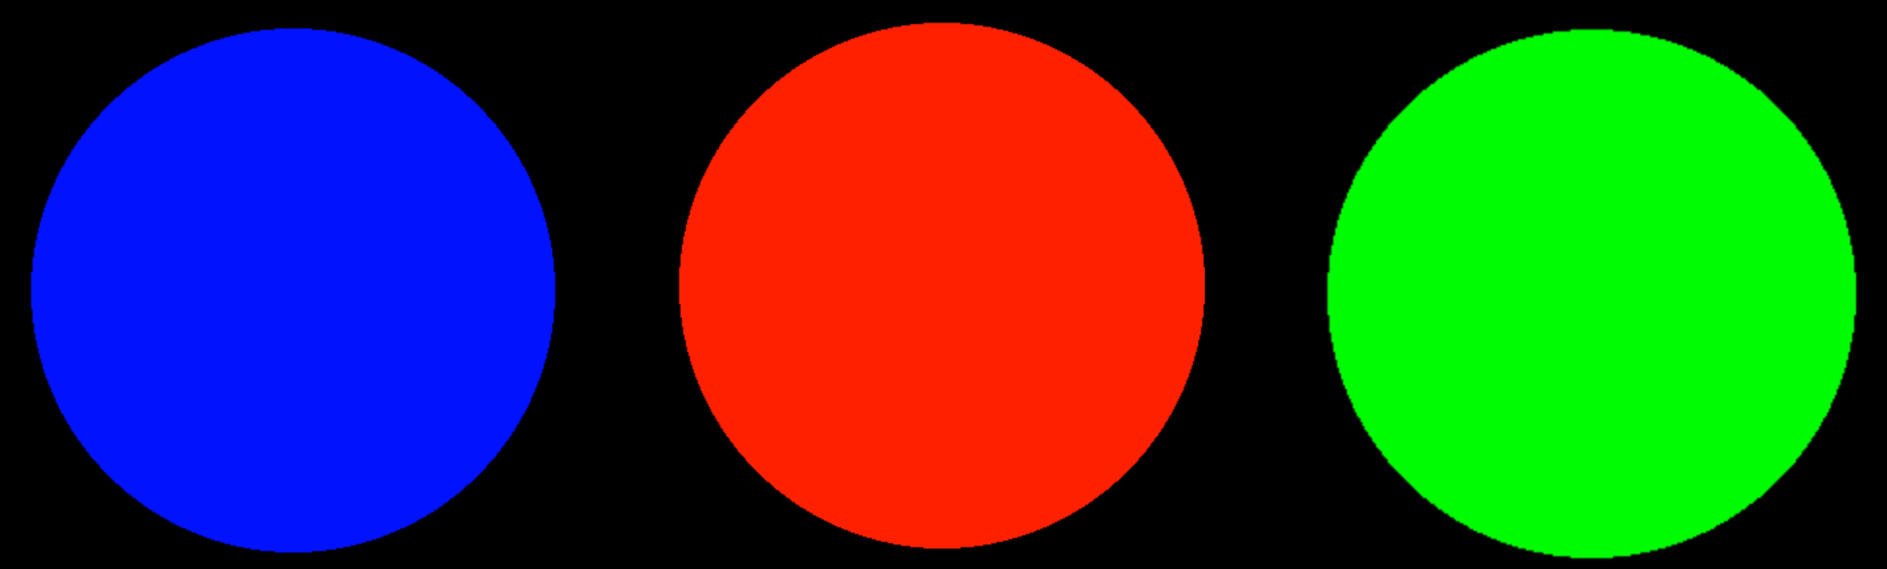
\includegraphics[width=10cm]{wdechwydechcisza}
\end{figure}
Jeżeli koło zwiększa się i jest niebieskie to model wykrywa wdech, jeśli zmniejsza się i jest
czerwone to jest to wydech, natomiast kolor zielony oznacza, że natężenie dźwięku nie przekracza pewnego 
progu dobieranego eksperymentalnie w zależności od mikrofonu.
Dalej klasyfikacja na żywo nazywana jest też testem jakościowym.
\section{Przyjęty model oddechu}
Na początku przyjmujemy model "sportowego" oddychania, czyli wdech nosem i wydech ustami.
Uproszczenie to polega na tym, że wydawane dźwięki są dosyć różne, dopiero potem sprawdzamy jak nasze podejście będzie się sprawować
przy innych metodach oddychania.
\begin{figure}[H]
	\centering
	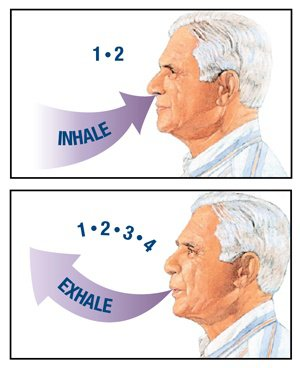
\includegraphics[width=3cm]{model_oddechu}
  	\caption{Ilustracja przyjętego modelu,  \href{https://www.quora.com/Should-I-exhale-from-the-mouth-or-nose-while-deep-breathing}{źródło}}
\end{figure}
\section{Średnia częstotliwość w czasie}
\subsection{Metoda}
Pierwotnie przyjętym założeniem było, że podczas wdechu średnia częstotliwość dźwięku jest wyższa niż
gdy osoba wydycha. Z pliku w formacie .wav pobieramy natężenie, które następnie\textbf{odszumiamy} za pomocą $noisereduce$ (przy testach jakościowych stosujemy bramkę szumów dla 3 ostatnich sekund) . 
\textbf{Dzielimy próbki na bloki, dla których tworzymy spektrogramy} i obliczamy
średnią ważoną częstotliwość.
Cechami, na podstawie których dokonywana jest predykcja są  
\begin{gather*}
\boldsymbol x (t_n) = [\bar{f}(t_0), \bar{f}(t_1), ..., \bar{f}(t_n)]
\end{gather*}
czyli średnie częstotliwości z kilku przeszłych chwil.
Dla danych testowych spełniających powyższe założenie i modelu wytrenowanego SVM-em dawało nam to dokładność $\sim 60\%$.
\begin{figure}[H]
	\centering
	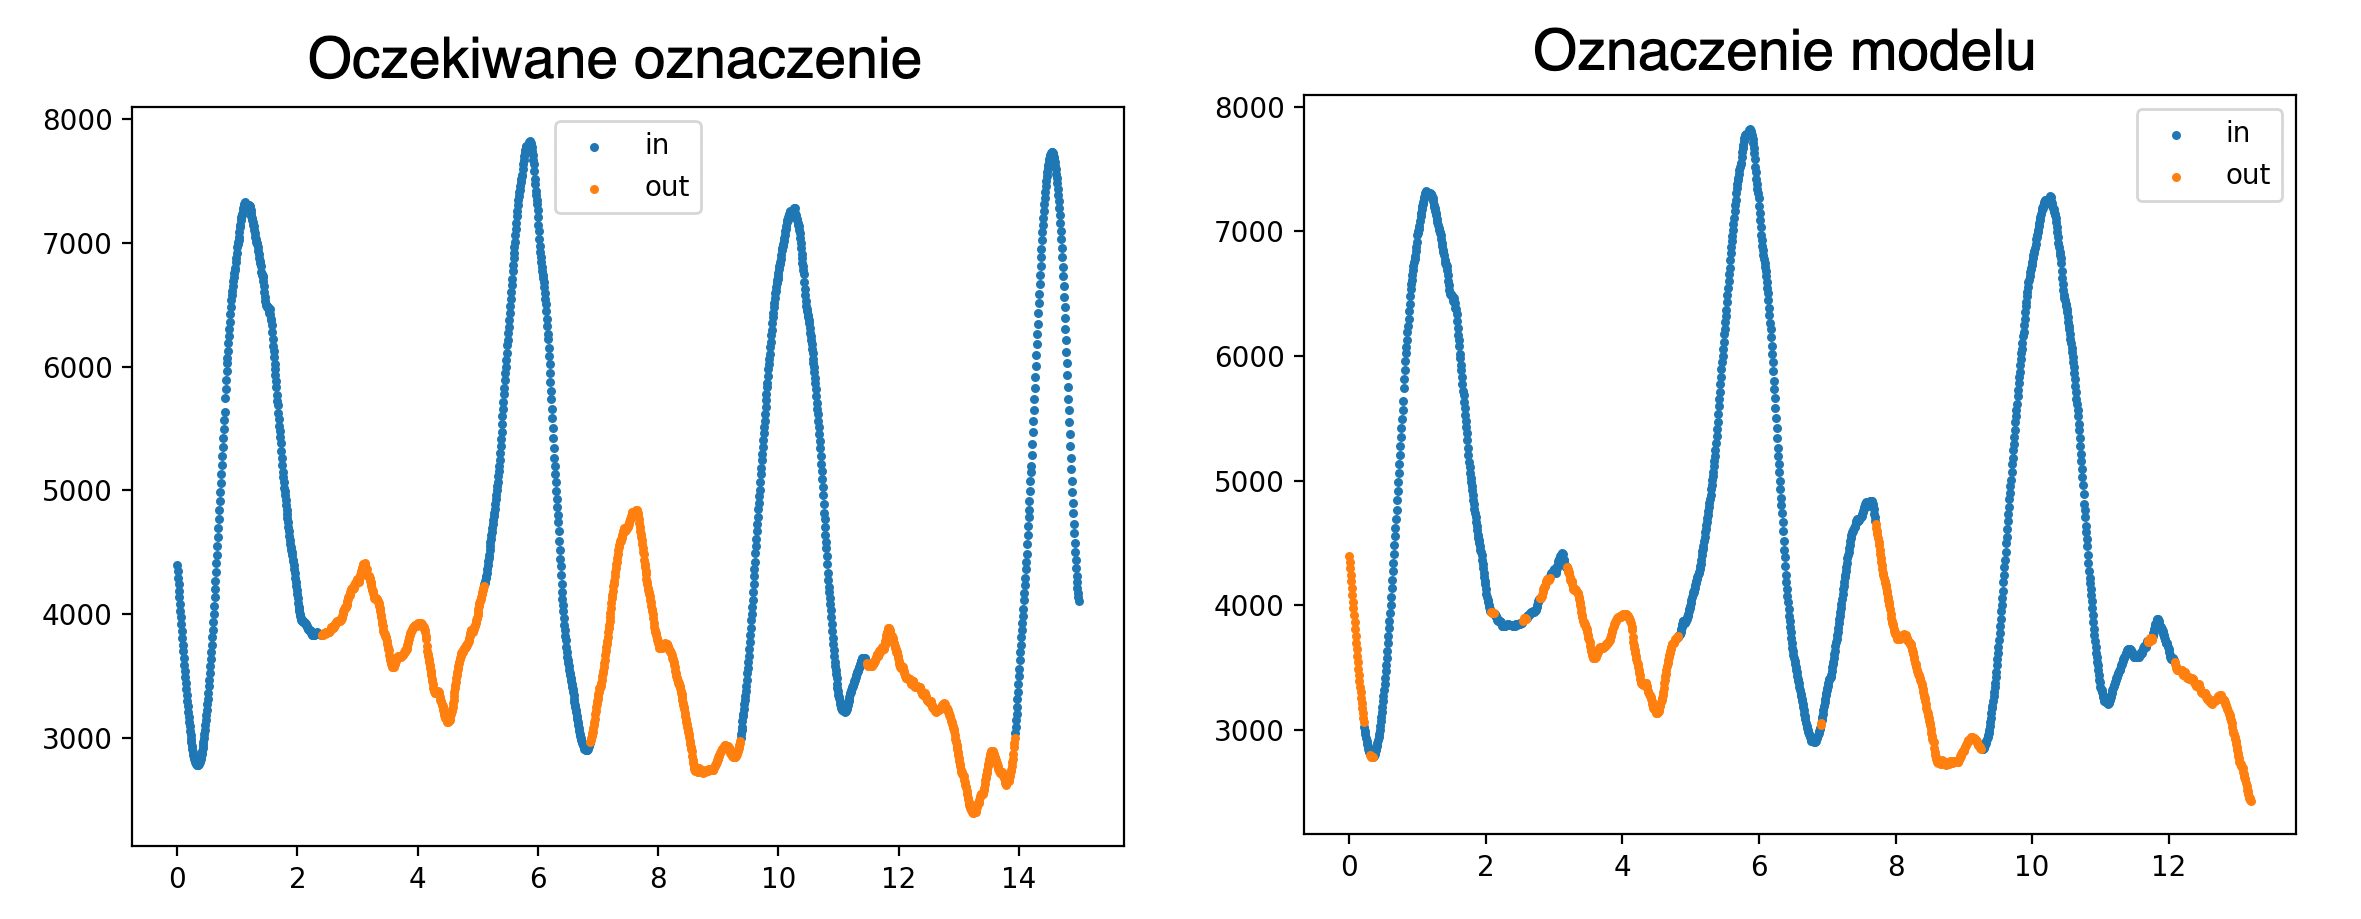
\includegraphics[width=10cm]{porownanie_srednie}
	\caption{Przykładowe działanie modelu dla danych spełniających założenie: wyższy wdech, niższy wydech.
	W pewnych momentach podobnie wyglądające fragmenty krzywej powinny być wdechem, w innych wydechem, mamy więc możliwy underfitting.}
\end{figure}
\subsection{Problemy}
Podejście to jednak mocno ograniczna nasze dalsze pole do rozwoju.  Zmniejszenie całego 
spektrogramu do pojedynczej wartości częstotliwości daje nam mniej informacji, przez co 
być może ograniczylibyśmy się tylko do przyjętego przez nas modelu (tj.  wdech - nos, wydech - usta) - w innych
modelach różnica średnich częstotliwości między wdechem a wydechem może nie być taka wyraźna.  Ponadto, dla niektórych osób zaobserwowaliśmy, 
że zależność między wdechem a wydechem jest niekoniecznie tak prosta jak założyliśmy. Obserwowana metoda
była również bardzo niestabilna jeżeli chodzi o testy jakościowe (klasyfikację na żywo).
\begin{figure}[H]
	\centering
	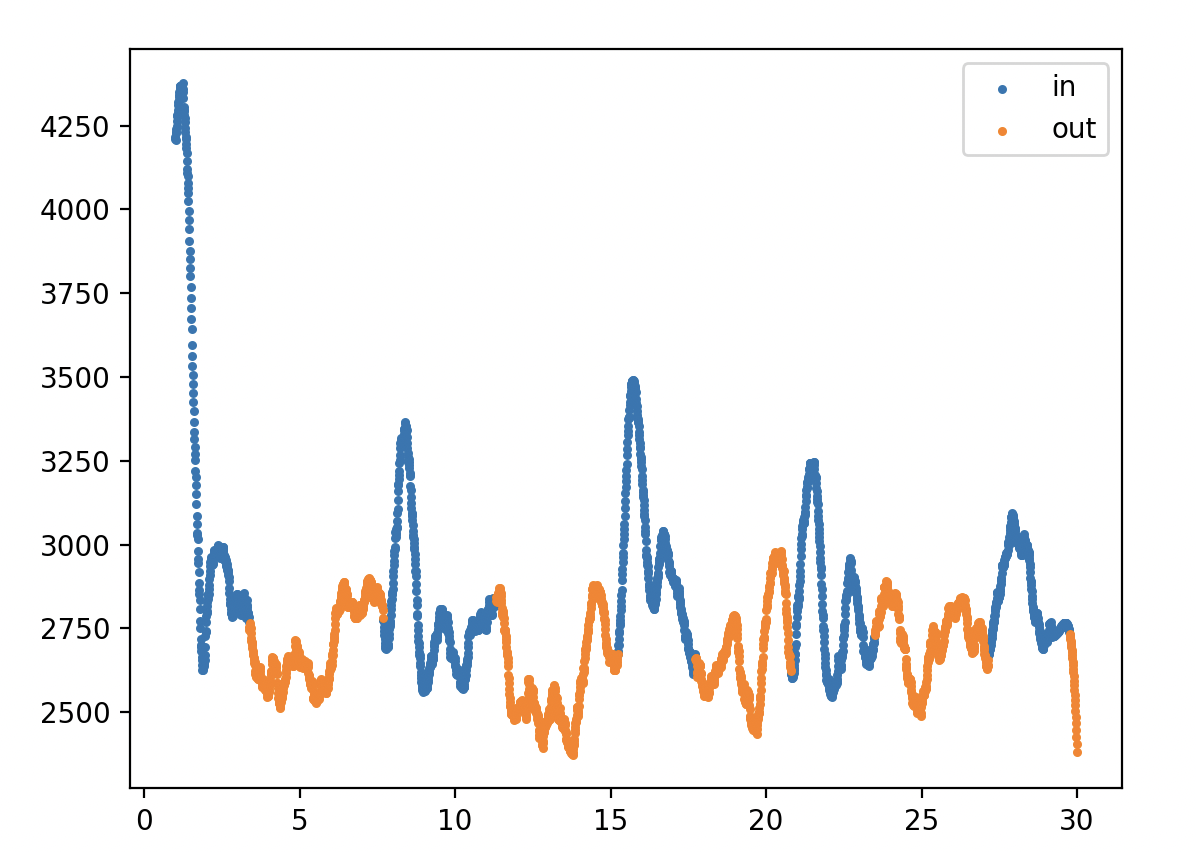
\includegraphics[width=10cm]{problem_srednie}
	\caption{Nieoczywista zależność między wdechem a wydechem.}
\end{figure}

\section{Dane wejściowe ze spektrogramu + SVM}
\subsection{Założenie}
Kolejnym przyjętym przez nas podejściem było wzięcie całego spektrogramu (a przynajmniej jego części) jako dane wejściowe do SVM-a.  
Metoda pochodzi od przypuszczenia, że człowiek rozpoznaje i rozróżnia wdech/wydech
na podstawie barwy dźwięku.  
\begin{figure}[H]
	\centering
	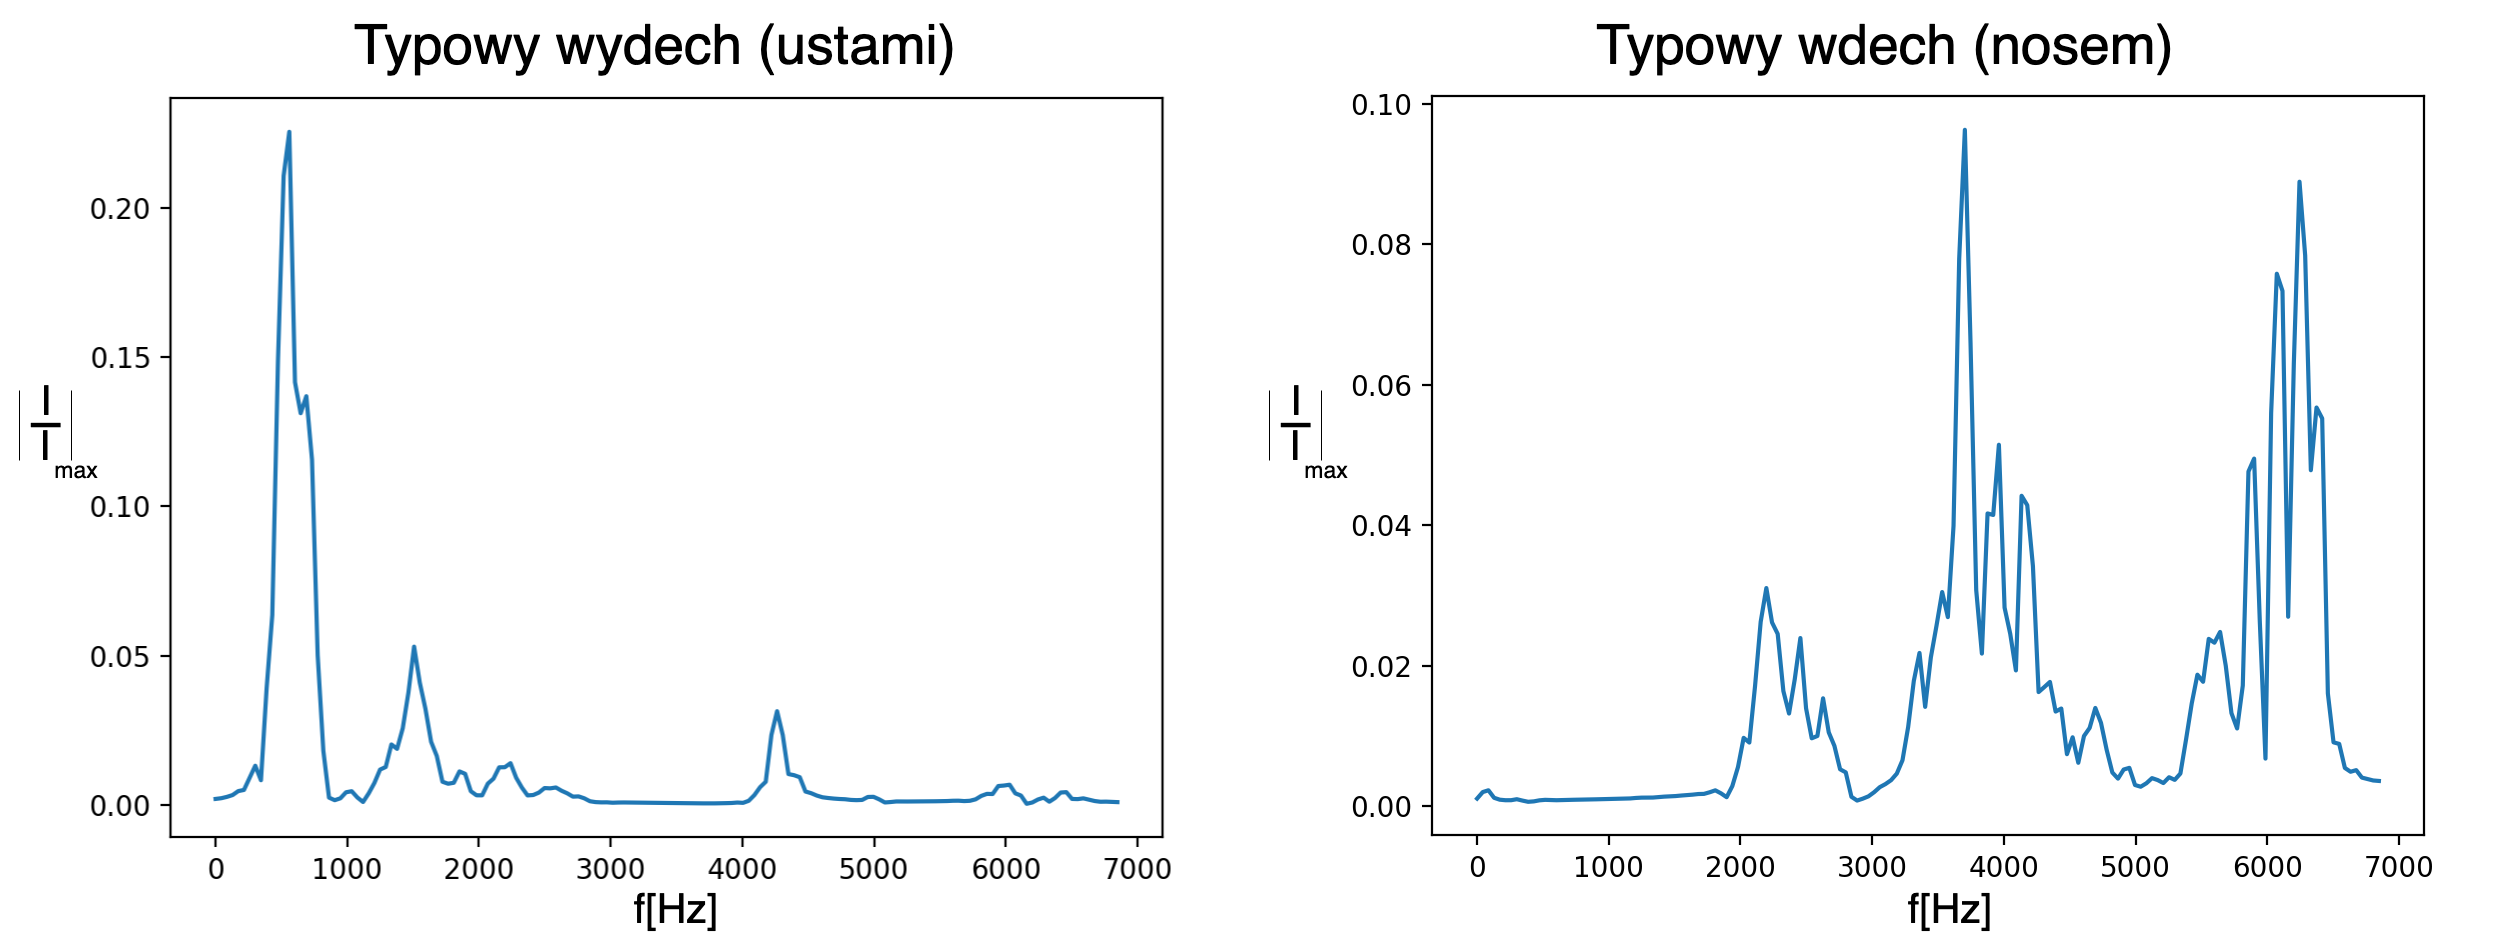
\includegraphics[width=10cm]{wdech_wydech_spektro}
  	\caption{Nie są istotne dokładne kształty powyższych spektrogramów, tylko fakt, że wydech
jest pojedynczym pikiem $\in (0, 1)$ kHz a wdech częstotliwościami z natężeniem
o mniejszym odchyleniu $\in (2, 7)$ kHz.  Zbliżoną zależność zaobserwowano dla paru osób.}.
\end{figure}
\subsection{Metoda}
Podobnie jak ostatnio pierw odszumiamy sygnał z pliku za pomocą $noisereduce$. \textbf{Dzielimy dane na bloki
rozmiaru 1024 próbek, tworzymy dla każdego bloku spektrogram} ale tym razem nie liczymy średniej tylko zostawiamy całą taką klatkę. Wektor cech ma więc postać 
\begin{gather*}
\boldsymbol{x} = [I_{f_1}, I_{f_2}, ..., I_{f_n}]
\end{gather*}
Nie są nam 
potrzebne wszystkie częstotliwości zwracane przez algorytm DFT, więc stosujemy ograniczenie podobne
do tego stosowanego w telefonii komórkowej -  \textbf{używamy 160 częstotliwości z przedziału do 6,9 kHz}.
Stosując to podejście dla danych testowych otrzymaliśmy $\sim 70\%$ dokładności. W testach
jakościowych jednak zaobserwować było można "przeskakiwanie" z jednej
wartości na drugą i spowrotem np. w połowie brania wdechu, wydychania.
\begin{figure}[H]
	\centering
	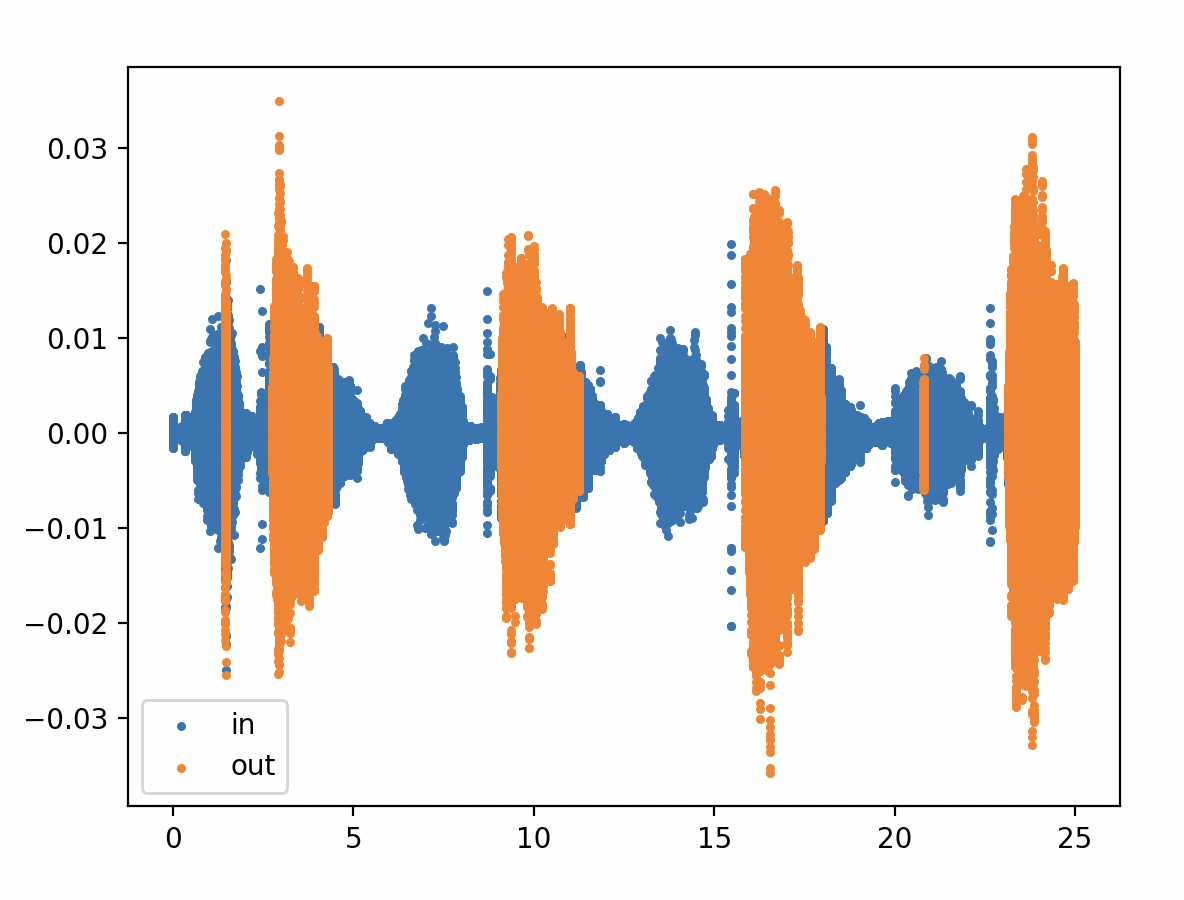
\includegraphics[width=10cm]{przeskakiwanie}
  	\caption{Dane z rysunku 1. oznaczone, jak widać, występują przeskoki z jednej wartości na drugą.}
\end{figure}

\subsection{Poprzedni stan}
W celu pozbycia się "przeskakiwania" i ogólnej poprawy działania dane z poprzedniego podpunktu rozszerzyliśmy o informację o \textbf{wcześniej przewidzianym stanie}, czyli 
\begin{gather*}
	\boldsymbol{x} = [I_{f_1}, I_{f_2}, ..., I_{f_160},  s]
\end{gather*}
 gdzie $s = 1$ jeśli poprzednio stwierdzono wdech, $s=-1$ jeśli poprzednio stwierdzono wydech.
Dodatkowo przeprowadziliśmy jeszcze \textbf{wygładzenie spektrogramu filtrem Savitzky-Golay}.
Takim sposobem otrzymaliśmy dokładność $\sim 99\%$ dla danych testowych w sytuacji idealnej - jako wartość $s$ stanu poprzedniego stosowaliśmy tą wziętą z
danych testowych, czyli zakładaliśmy za każdym razem, że nasz model przewidzi dobrze poprzedni stan.
Przypadek ten nie jest realny, ponieważ model nie będzie znał poprawnej poprzedniej klasyfikacji tylko 
zakładał, że to co sam stwierdził jest poprawne.  Biorąc poprzedni stan nie z danych testowych a z poprzedniej
klasyfikacji modelu otrzymujemy mniejszą dokładność $\sim 80\%$. Wniosek z tego jest taki, że model
z wysokim prawdopodobieństwem przewidzi dobrze kolejny stan, jeżeli dobrze porzewidział poprzedni. 
Warto dodać, że rzeczywiście metoda z poprzednim stanem pozwoliła nam ograniczyć "przeskakiwanie" 
w testach jakościowych.
\subsection{Problemy}
W poprzednim podpunkcie wyszedł główny mankament tej metody - konieczność założenia, że poprzednio
przewidziany stan jest dobry co nie zawsze jest prawdą. W testach jakościowych zaobserwować można było
"wariowanie" modelu, czyli sekwencję źle przewidzianych stanów.

\section{Spektrogram i sieć neuronowa}

\section{Przejście na inny model oddychania}
Kolejnym krokiem będzie przeniesienie wyżej wspomnianych metod na model oddychania nos-nos. 
Będzie to być może wymagało wzięcia innych częstotliwości.

\section{Działanie modelu a hałas z otoczenia}

\section{Douczanie}

\section{Wnioski}

\section{Źródła}
\begin{thebibliography}{2}
\bibitem{Cormen} 
 Cormen Thomas H., Leiserson Charles E., Rivest Roland L., Stein Clifford (1989) \emph{Wprowadzenie do algorytmów},
\bibitem{DFT}
\url{https://pl.wikipedia.org/wiki/Dyskretna_transformata_Fouriera}
\bibitem{Bramkaszumow}
Kumar, E. and Surya, K. and Varma, K. and Akash, A. and Kurapati, Nithish Reddy (2023) \emph{Noise Reduction in Audio File Using Spectral Gatting and FFT by Python Modules}
\bibitem{SavgolImage}
\url{https://www.maplesoft.com/Applications/Detail.aspx?id=154593}
\end{thebibliography}



\end{document}
